%%%%%%%%%%%%%%%%%%%%%%%%%%%%%%%%%%%%%%%%%%%%%%%%%%%%%%%%%%%%%%%%%%
%%%%%%%%%%%%%%%%%%%%%%%%%%%%%%%%%%%%%%%%%%%%%%%%%%%%%%%%%%%%%%%%%%
% Packages
\documentclass[10pt, a4paper]{article}
\usepackage[ngerman]{babel}
\usepackage[top=3cm, bottom=4cm, left=3.5cm, right=3.5cm]{geometry}
\usepackage{amsmath,amsthm,amsfonts,amssymb}
\usepackage{color}
\usepackage{graphicx}
\usepackage{float}
\usepackage[dvipsnames]{xcolor}
\usepackage{fancyhdr}
\usepackage{hyperref}
\usepackage{url}

%%%%%%%%%%%%%%%%%%%%%%%%%%%%%%%%%%%%%%%%%%%%%%%%%%%%%%%%%%%%%%%%%%
%%%%%%%%%%%%%%%%%%%%%%%%%%%%%%%%%%%%%%%%%%%%%%%%%%%%%%%%%%%%%%%%%%
% Define colors
\definecolor{htmlgreen}{HTML}{009879}
\definecolor{htmlred}{HTML}{bb1004}
\definecolor{htmlblue}{HTML}{80b8f8}
\definecolor{htmlviolet}{HTML}{d1aeee}

%%%%%%%%%%%%%%%%%%%%%%%%%%%%%%%%%%%%%%%%%%%%%%%%%%%%%%%%%%%%%%%%%%
%%%%%%%%%%%%%%%%%%%%%%%%%%%%%%%%%%%%%%%%%%%%%%%%%%%%%%%%%%%%%%%%%%
% Code display
\usepackage{minted}
\usemintedstyle{autumn}

%%%%%%%%%%%%%%%%%%%%%%%%%%%%%%%%%%%%%%%%%%%%%%%%%%%%%%%%%%%%%%%%%%
%%%%%%%%%%%%%%%%%%%%%%%%%%%%%%%%%%%%%%%%%%%%%%%%%%%%%%%%%%%%%%%%%%
% Page setup
\pagestyle{fancy}
\headheight 35pt
\lhead{\today}
\rhead{
\includegraphics[width=2.5cm]{pictures/Goethe_University_logo.jpg}}
\lfoot{Seminar Datenkompression}
\pagenumbering{arabic}
\cfoot{\small\thepage}
\rfoot{Goethe-Universität}
\headsep 2.2em

%%%%%%%%%%%%%%%%%%%%%%%%%%%%%%%%%%%%%%%%%%%%%%%%%%%%%%%%%%%%%%%%%%
%%%%%%%%%%%%%%%%%%%%%%%%%%%%%%%%%%%%%%%%%%%%%%%%%%%%%%%%%%%%%%%%%%
% Title page
\begin{document}

\begin{titlepage}
    \begin{center}
        \vspace*{3cm}
            
        \Huge
        \textbf{Seminar Datenkompression}
            
        \vspace{1cm}
        \huge
        ZIP-Verfahren: LZ77-Algorithmus
            
        \vspace{1.5cm}
        \Large
            
        \textbf{Tobias Völkner 5328855}\\  % <-- author1
        \textbf{Philipp Stephan 7182981}    % <-- author2
        
            
        \vfill
        
        Dozent: Dr.- Ing. The Anh Vuong\\
        Graphische Daten Verarbeitung, Informatik Institut\\
        Johann Wolfgang Goethe Universität, Frankfurt am Main

            
        \vspace{1cm}
            
        
\includegraphics[width=0.4\textwidth]{pictures/Goethe_University_logo.jpg}
        \\
        
        \Large
        
        \today
            
    \end{center}
\end{titlepage}

%%%%%%%%%%%%%%%%%%%%%%%%%%%%%%%%%%%%%%%%%%%%%%%%%%%%%%%%%%%%%%%%%%
%%%%%%%%%%%%%%%%%%%%%%%%%%%%%%%%%%%%%%%%%%%%%%%%%%%%%%%%%%%%%%%%%%
% Document begin
\newpage
\tableofcontents
\newpage

\section{Datenkompression}
Datenkompression oder Datenkomprimierung ist ein Vorgang der Menge von digitalen Daten reduziert. Dadurch soll weniger Speicherplatz benötigt und die Übertragungszeit der Daten verringert werden. Der grundsätzliche Ansatz ist dabei, redundante bzw. nicht notwendige Informationen zu entfernen und Daten in verkürzter Form darzustellen. Dieser Vorgang wird Komprimierung genannt. Der umgekehrte Vorgang wird als Dekomprimierung bezeichnet. Dabei werden die reduzierten Daten wieder in ihren lesbaren Zustand zurückgesetzt. \\

\noindent
Die Datenkomprimierung unterliegt gewissen Grenzen, da die Daten nicht beliebig gekürzt werden können. Deshalb unterscheidet man zwischen zwei Arten von Komprimierung: Die verlustfreie Kompression, bei der die Originaldaten ohne Verlust von Informationen aus den komprimierten Daten zurückgewonnen werden können, und die verlustbehaftete Kompression, bei der ein Teil der Informationen während der Komprimierung verloren geht. \cite{website:kompression}

\subsection{Verlustfreie Kompression}
Bei der verlustfreien Kompression muss gewährleistet sein, dass aus den komprimierbaren Daten die Originaldaten wiederhergestellt werden können. Es gehen also keine Informationen verloren. Verlustfreie Kompressionsverfahren nutzen oft die Redundanz, also das mehrfache Vorkommen, von Daten aus.Verlustfreie Kompression wird deshalb auch als Redundanzreduktion bezeichnet. Der Algorithmus zum Dekomprimieren zählt dabei zu den komprimierten Daten hinzu, da die komprimierte Datei sonst wertlos wäre. Ohne eine erkennbare Struktur oder Besonderheiten, ist keine Komprimierung möglich. Verlustfreie Kompression findet oft bei der Komprimierung von Texten Anwendung. \cite{website:kompression}

\subsection{Verlustbehaftete Kompression}
Bei der verlustbehafteten Kompression werden redundante/irrelevante Informationen ausgelassen, um somit die Datengröße zu reduzieren. Es wird deshalb auch von Irrelevanzreduktion gesprochen. Was als "redundant" gilt, unterscheidet sich dabei je nach Anwendungsfall. Die Schwelle dafür kann bis zu einer Größe von einem Bit heraufgesetzt werden. Ein Modell entscheidet welche Informationen für den Empfänger wichtig sind, und welche nicht. Verlustbehaftete Kompression wird meist bei Bild-, Audio-, oder Videodateien und -übertragungen angewandt. \cite{website:kompression}

\newpage
\section{Theoretische Grundlagen}
In der Datenkompression gibt es verschiedene Methoden, Algorithmen und Dateiformate. Im Folgenden werden einige Grundlagen für den LZ77-Algorithmus erklärt.

\subsection{Die Wörterbuchmethode}
Die Wörterbuchmethode ist eine Art der verlustfreien Kompression. Bei diesem Verfahren werden wiederkehrende Zeichen oder Zeichenketten durch Abkürzungen, sogenannte Tokens, ersetzt. Um die Tokens den zugehörigen Zeichen(-ketten) zuordnen zu können, wird ein Wörterbuch angelegt. Dieses Wörterbuch muss in den komprimierten Daten mit aufgenommen werden, damit die ursprünglichen Daten wieder hergestellt werden können. Diese Methode ist besonders nützlich, wenn sich eine kleine Anzahl
Muster sehr häufig im Text wiederholt. Wörterbuchmethoden werden in zwei Kategorien unterteilt. Wenn es genügend Kenntnis über den Text gibt, wird ein statisches Verfahren - mit einem festen Wörterbuch - verwendet. Ist das nicht der Fall, wird ein dynamisches Verfahren eingesetzt, bei dem das Wörterbuch im Laufe der Codierung erstellt wird. Ein großer Vorteil der Wörterbuch-Techniken ist, dass ganze Zeichenketten codiert werden können und nicht nur einzelne Zeichen. \cite{website:woerterbuch, website:uni-trier}

\paragraph{Statische Verfahren}
Statische Wörterbuch-Verfahren sind in der Regel nur für spezielle Fälle sinnvoll. Das ist dann der Fall, wenn Zeichen bzw. Zeichenketten sehr häufig vorkommen, beispielsweise Dateien, in denen Leistungen von Studenten erfasst sind. Wörter wie ''Vorname'', ''Nachname'', ''Matrikelnummer'' und ''Note'' kommen dort sehr häufig vor. \cite{website:uni-trier}

\paragraph{Dynamische Verfahren}
Bei dynamischen Verfahren wird das Wörterbuch erst bei der Codierung erstellt. Es wird also vorher keine Kenntnis über den Text benötigt und das Wörterbuch enthält nur die Informationen die auch gebraucht werden. \cite{website:uni-trier}

\subsection{Das ZIP-Dateiformat}
Das ZIP-Dateiformat ist ein Dateiformat für verlustfrei komprimierte Daten und dient zur Archivierung oder zum Versand von Dateien. Das erste ZIP-Dateiformat wurde 1989 vom US-Amerikaner Phil Katz mit dem Programm PKZIP für die Kompression und PKUNZIP für die Dekompression entwickelt. Weitere ZIP-Formate basieren auf dieser ersten Herausgabe. 
Die Kompression in einer ZIP-Datei reduziert die Größe der Ursprungsdaten bei der Archivierung und wird als Containerformate gespeichert. Alle Dateien werden individuell komprimiert und dann der Archiv-Datei zusammengefasst. Für das ZIP-Dateiformat gibt es verschiedene Kompressions-Algorithmen. Einer der bekanntesten ist der LZ77- Algorithmus von Abraham Lempel und Jacob Ziv. \cite{website:zip}

\newpage
\section{Der LZ77-Algorithmus}
LZ77 ist ein Verfahren zur verlustfreien Kompression von Daten. Es wurde 1977 von Abraham Lempel und Jacob Ziv im Fachmagazin ''IEEE Transactions of Information Theory'' veröffentlicht (daher der Name "Lempel-Ziv-1977"). Es handelt sich hierbei um ein Wörterbuch-Verfahren, welches sich als erstes seiner Art mehrfach auftauchende, ganze Sequenzen an Zeichen in einem Datensatz zunutze macht, anstatt die Wahrscheinlichkeiten für das Auftreten von Zeichen oder Zeichenfolgen zu verwenden (Entropiekodierung). Es ist das erste von vielen darauf folgenden LZ-Verfahren und bildete die Grundlage für weitere Kompressionsverfahren und viele Varianten, mit denen die Kompressionsrate weiter verbessert wird. \\

\noindent
Das Ziel von Lempel und Ziv war es einen Algorithmus zu entwickeln, der ohne Vorkenntnisse über den Text und ohne Voruntersuchung der Eingabe, effektiv komprimiert. Der LZ77-Algorithmus liest die Daten nur ein einziges mal, die Eingabe erfolgt zeichenweise und baut auf den vorher eingelesenen Teilen des Datenstroms auf. Daraus folgt der Vorteil die Daten Stück für Stück verarbeiten zu können, auch wenn diese noch nicht vollständig zur Verfügung stehen. Da keine Voranalyse der zu komprimierenden Daten stattfindet, ist die Kompression nicht immer zwangsläufig optimal. Im schlimmsten Fall kann aufgrund weniger Redundanzen sogar eine Vergrößerung der Datenmenge auftreten. \\

\noindent
Da Zeichenfolgen nur dann ersetzt werden können, wenn diese vorher schon einmal aufgetreten sind, ist die Kompressonsrate anfangs noch sehr gering und der Algorithmus liefert erst mit fortschreitendem Einlesen der Eingabedaten bessere Ergebnisse. Daraus folgt, dass zu kleine Eingabestrings zu schlechten Kompressionsraten führen. \cite{website:uni-duisburg-essen, website:lz77, website:rwth-aachen}

\subsection{Kompressionsvorgang}
Ein Eingabe-Text wird komprimiert, indem man nach sich wiederholenden Zeichenketten sucht und diese durch eine Referenz ersetzt, die auf das Original verweist. Diese Referenzen werden anschließend in einem Wörterbuch gespeichert. Falls ein Zeichen zum ersten Mal auftaucht, wird dieses im Wörterbuch ohne Referenz gespeichert. Dabei wird der Eingabetext zeichenweise durch einen Buffer, das sogenannte Sliding Window, bewegt. Dieses Sliding Window ist unterteilt in den Search-Buffer und den Lookahead-Buffer. Der Search-Buffer ist dabei üblicherweise mehrere Tausend Zeichen lang, der Lookahead-Buffer mehrere Hundert Zeichen. \\

\noindent
Der Algorithmus durchläuft dabei den Text, definiert als Zeichenkette $Z = {s_1,...,s_k}$, und sucht für jedes Symbol $s_i \in Z$, ein Match in der Zeichenkette $Z_i = s_{i-1},...,s_{i-x}$. Dabei gilt $x \leqslant i \leqslant k$. Die Zahl $x$ ist die Länge des Search-Buffers, der die Zeichenkette $Z_i$ rückwärts durchläuft. \newline
Der Searchbuffer durchsucht dabei den Text rückwärts, ausgehend des aktuellen Symbols, nach einem Match. Bei Fund eines Matches zweier Symbole $s_i$ und $s_j:(i-x \leqslant j < i)$ wird, mithilfe des Lookahead-Buffers der Länge $l$, geprüft ob eine Sequenz existiert. \newline Für ein Match einer Sequenz wird ein Tupel der Form $(offset,\; length,\; nextSymbol)$ erstellt, definiert als: 
\begin{itemize}
    \item $offset :=$ der Abstand zwischen den jeweils ersten Symbolen der beiden Sequenzen
    \item $length :=$ die Länge der Sequenz
    \item $nextSymbol :=$ das nächste Symbol nach Abschluss der Sequenz
\end{itemize} 

\noindent
Die Funktion für eine gefundene Sequenz der Länge $m \leqslant l$ liest sich daher wie folgt:
\begin{center}
    $s_j,...,s_{j+m} = s_i,...,s_{i+m} \Rightarrow (i-j,m,s_{i+m+1})$\newline
\end{center}
Für den Fall, dass sich keine Sequenz finden lässt, wird folgendes Tupel $t$ erstellt:
\begin{center}
    $(0,0,s_i)$
\end{center}

\noindent
Die Tupel werden anschließend, in Reihenfolge, in ein Wörterbuch $L:=t_1,...,t_g$ eingetragen. \\

\noindent
Die Effektivität der Kompression des LZ77-Algorithmus hängt hauptsächlich von der Größe des Sliding Window ab. Ein kleinerer Search-Buffer führt zu weniger gefundenen Übereinstimmungen. Ein kleinerer Lookahead-Buffer führt zu kürzeren Übereinstimmungen. Bei kleinen Buffer-Größen ist die Kompressionsrate also üblicherweise gering. Werden die Buffer allerdings zu groß gewählt, bedeutet das einen höheren Bedarf an Arbeitsspeicher und die Laufzeit der Suche nach Übereinstimmungen verlängert sich. \cite{website:uni-duisburg-essen}

\vspace{5mm}
\paragraph{Pseudocode}
Das Vorgehen des LZ77-Algorithmus bei der Kompression, dargestellt in Pseudocode. Im Anhang \ref{sec:encode} befindet sich eine vollständige Implementierung in der Programmiersprache Javascript.
\begin{minted}{js}
 while der Lookahed Buffer ist nicht leer;
     durchsuche rückwärts den Text nach der längsten 
            übereinstimmenden Zeichenkette mit dem Lookahead Buffer;
     
     if eine Übereinstimmung wurde gefunden;
         füge das Tripel (Versatz zum Rand des Lookahead Buffers,
                          Länge der gefundenen Zeichenkette,
                          erstes nicht übereinstimmendes Zeichen aus dem Lookahead Buffer)
                dem Wörterbuch hinzu;
         verschiebe das Sliding Window um die Länge+1;
     else
         füge das Tripel (0,
                          0, 
                          erstes Zeichen im Lookahead Buffer) 
                dem Wörterbuch hinzu;
         verschiebe das Sliding Window um 1;
\end{minted}

\vspace{5mm}
\paragraph{Beispiel}
Codierung des Textes ''abracadabra!''. Die linke Spalte der Tabelle symbolisiert den Search-Buffer mit der Größe 12, die Mittlere den Lookahead-Buffer mit der Größe 4 und die Rechte das Wörterbuch. Gefundene Übereinstimmungen sind \underline{unterstrichen} geschrieben.

\begin{table}[H]
    \centering
    \begin{tabular}{r|c|l|c}
        \multicolumn{3}{c|}{Sliding Window} & Wörterbuch \\
        Search-Buffer & \multicolumn{2}{l|}{Lookahead-Buffer} & \\
        \hline
         & a b r a & c a d a b r a ! & (0, 0, a) \\
        \hline
        a &  b r a c & a d a b r a ! & (0, 0, b) \\
        \hline
        a b & r a c a & d a b r a ! & (0, 0, r) \\
        \hline
        \underline{a} b r & \underline{a} c a d & a b r a ! & (3, 1, c) \\
        \hline
        a b r \underline{a} c & \underline{a} d a b & r a ! & (2, 1, d) \\
        \hline
        \underline{a b r a} c a d & \underline{a b r a} & ! & (7, 4, !) \\
        \hline
        a b r a c a d a b r a ! & & \\
        \hline
    \end{tabular}
    \caption{Veranschaulichung der Kompression.}
    \label{tab:codierung}
\end{table}

\newpage
\subsection{Dekompressionsvorgang}
Für die Dekompression wird das Wörterbuch ausgeschrieben. Dabei ist das Wörterbuch definiert als $L:=t_1,...,t_k$ und Tupel $t:=(offset,\; length,\; nextSymbol)$. Für jedes Tupel aus dem Wörterbuch wird ein entsprechender Text generiert. Für den Fall, dass $offset$ und $length$ beide 0 sind, wird nur $nextSymbol$ geschrieben. Das erste Tupel eines Wörterbuchs wird immer der Form $(0,\; 0,\; nextSymbol)$ sein und setzt damit den initialen Text $T:=z_1$. \\

\noindent
Typischerweise werden die ersten Tupel keine Referenzen enthalten. Jeder neu generierte Textabschnitt wird dann an $T$ angefügt. Wenn ein Tupel mit einer Referenz auf eine Zeichenkette gefunden wird, wird diese im aktuellen $T$ gesucht. Dabei wird die Zeichenkette $z_{l-offset},...,z_{l-offset+length}$ wiederholt und an $T$ gefügt. \\

\noindent
Zum Schluss wird $nextSymbol$ an die Zeichenkette gefügt. Sollte $nextSymbol$ leer sein, bleibt $T$ unverändert und dies bedeutet immer, dass der letzte Tupeleintrag erreicht wurde. 

\vspace{5mm}
\paragraph{Pseudocode}
Das Vorgehen des LZ77-Algorithmus bei der Dekompression, dargestellt in Pseudocode. Im Anhang \ref{sec:decode} befindet sich eine vollständige Implementierung in der Programmiersprache Javascript.
\begin{minted}{js}
for jedes Tripel (Versatz, Länge, Zeichen);
     if Länge > 0;
         durchlaufe rückwärts die bisherige Ausgabe und gib solange Zeichen aus
                 bis Länge erreicht ist,
                 bei einem Überlauf beginne erneut bei Versatz;
     Gib Zeichen aus;
\end{minted}

\vspace{5mm}
\paragraph{Beispiel}
Decodierung des in Tabelle \ref{tab:codierung} erstellten Wörterbuchs. \underline{Unterstrichen} geschriebene Buchstaben sind die für die Rekonstruktion verwendeten Buchstaben.
\begin{table}[h]
    \centering
    \begin{tabular}{l|l}
        Wörterbuch & Text \\
        \hline
        (0, 0, a) & a \\
        \hline
        (0, 0, b) & a b \\
        \hline
        (0, 0, r) & a b r \\
        \hline
        (3, 1, c) & \underline{a} b r \underline{a} c \\
        \hline
        (2, 1, d) & a b r \underline{a} c \underline{a} d \\
        \hline
        (7, 4, !) & \underline{a b r a} c a d \underline{a b r a} ! \\
        \hline
    \end{tabular}
    \caption{Veranschaulichung der Dekompression.}
\end{table}

\subsection{Speichereinsparung}
Bei der Kompression wird für die Tupel-Einträge unterschiedlich viel Platz alloziert, je nach dedizierter Länge der Buffer. Für die Länge der Buffer werden entsprechend viele Bits alloziert. Dabei würde im oben genannten Beispiel (''abracadabra!'')  für einen Search-Buffer der Länge 12, $\lceil \log_2(12) \rceil =$ 4 Bits alloziert und für einen Lookahead-Buffer der Länge 4, $\lceil \log_2(4) \rceil =$ 2 Bits. Für die Symbole wird im Normalfall 1 Byte, also 8 Bits alloziert. Das Wort ''abracadabra!'' enthält insgesamt 12 Symbole, damit 96 Bits. Das entsprechende Wörterbuch enthält 6 Einträge, also $6 \cdot (4+2+8) \text{ Bits} = 84 \text{ Bits}$. Damit hätte man für das Beispiel eine Einsparung von insgesamt 12 Bits. Die Speichereinsparung verändert sich dynamisch, je nach Textart, Bufferlänge und Textlänge. \cite{website:FU-Berlin}


\section{Anwendungsgebiet}
Das LZ77-Verfahren wird heutzutage nur noch selten verwendet. Allerdings ist es die Grundlage für viele, darauf aufbauende Kompressionsalgorithmen, wie, unter anderem, der LZ78-Algorithmus von 1978, der Lempel-Ziv-Storer-Szymanski-Algorithmus (LZSS), der Lempel-Ziv-Welch-Algorithmus (LZW) und die Lempel-Ziv-Markov-Kompression (LZMA). \\

\noindent
Die Nachfahren des LZ77 finden in vielen Bereichen noch heute Anwendungen, zum Beispiel: Gif, PDF, TIFF, im Unix-'compress' command und vielen mehr. Das eigentliche LZ77-Verfahren wird heutzutage zum Beispiel noch auf dem Game Boy Advance, dem AutoCAD DWG Format und weiteren eingebetteten Systemen verwendet. Kombiniert mit der Huffman-Kodierung wird LZ77 im häufig verwendeten Deflate-Algorithmus angewandt. Dieser wird unter anderem vom Grafikformat PNG und anderen sehr bekannten Kompressionsprogrammen eingesetzt. In der algorithmischen Verarbeitung von Zeichenketten wird LZ77 außerdem zur Erkennung von Regelmäßigkeiten in Strings genutzt. Da die Weiterentwicklungen allgemein effizienter sind, werden diese heutzutage meist der LZ77-Kompression bevorzugt. \cite{website:kompression}

\section{Qualitätsbewertung}
\paragraph{Vorteile}
Das LZ77-Verfahren hat den großen Vorteil, dass es ohne Textkenntnis komprimieren kann. Des Weiteren ist es mit keinem Patent belegt, was bedeutet, dass die Verwendung des Algorithmus' sehr unkompliziert ist. LZ77 kommt außerdem mit wenig Systemressourcen aus und liefert dafür hinreichende Ergebnisse. Der Algorithmus dient zudem heutzutage oft als Ausgangspunkt, um neue Algorithmen zu entwerfen, da er recht einfach zu erlernen, zu programmieren und zu erweitern ist. Mit Variationen des Algorithmus lassen sich somit sehr effektive Kompressionsverfahren erstellen, die mit den heutigen komplexen Verfahren auf einem Niveau sind.

\paragraph{Nachteile}
Ein offensichtlicher Nachteil des Verfahrens ist, dass bei wenigen Wiederholungen innerhalb des Textes oder der Zeichenkette nur wenige Referenzen erstellt werden können oder die Datenmenge im worst-case sogar vergrößert werden kann. Das ist insbesondere bei kleinen oder nicht natürlichsprachigen Texten der Fall. Des Weiteren werden beinahe ausschließlich Zeichenfolgen genutzt, die sich nah um den Zeiger der aktuellen Iteration befinden, da der Lookahead- und Search-Buffer die Reichweite der gefundenen Matches limitieren. Diese Buffer sind natürlich unendlich erweiterbar, allerdings mit Befall massiver Kosten der CPU-Laufzeit bei der Kompression und Auswirkung auf die Speichergröße der Tupel durch die größere Bufferlänge.

\paragraph{Fazit}
Der LZ77-Algorithmus dient heutzutage eher als sogenannter Präprozessor, also der Vorverarbeiten des Textes, um danach mit einem anderen Kompressionsverfahren (beispielsweise der Huffman-Kodierung) stärker zu komprimieren oder er dient als Grundlage, dafür neue, mächtigere Kompressionsalgorithmus zu entwickeln. \cite{website:fh-koeln,website:wikibooks,website:lz77,website:Stanford-Engineering}

\newpage
\section{Demonstrations-Kit}
Das Demonstrations-Kit besteht aus drei Bereichen. Ein Bereich für die Eingabe, ein weiterer für die Visualisierung der Kompression und ein letzter für die Visualisierung der Dekompression.

\begin{figure}[H]
    \centering
    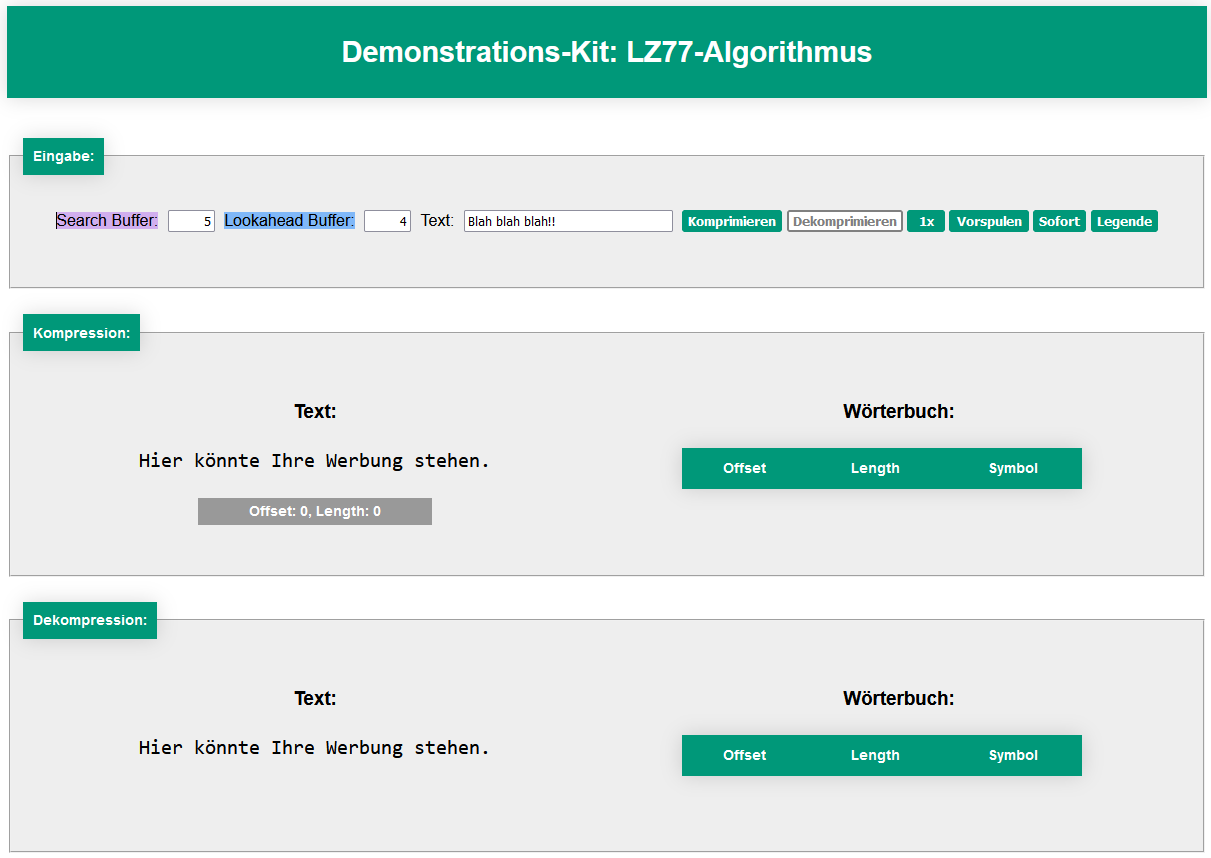
\includegraphics[scale=0.45]{pictures/DemonstrationsKit.png}
    \caption{Oberfläche des Demonstrations-Kit.}
\end{figure}

\noindent
Im Eingabe-Bereich lässt sich die Größe des Search- und Lookahead-Buffers festlegen, sowie einen Text von bis zu 1000 Zeichen eingeben. Dieser Text wird dann komprimiert bzw. dekomprimiert. Der Button zum Dekomprimieren wird erst nach der Komprimierung freigeschaltet. Zusätzlich lässt sich mit je einem Button die Geschwindigkeit der Visualisierung regeln, vorspulen oder sie sofort beenden.

\begin{figure}[H]
    \centering
    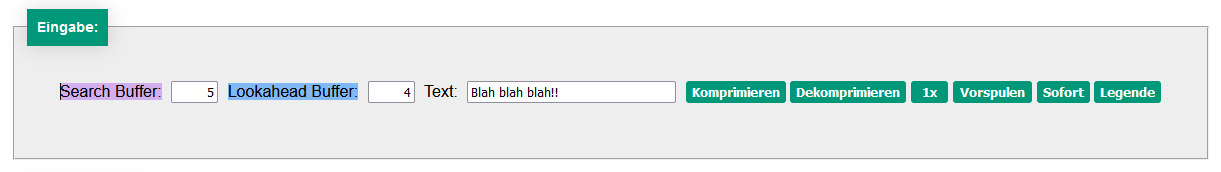
\includegraphics[scale=0.45]{pictures/Eingabe.png}
    \caption{Eingabe-Bereich des Demonstrations-Kit.}
\end{figure}

\noindent
Der Kompressions-Bereich stellt die Kompression des LZ77-Algorithmus visuell anschaulich dar. Hier wird auf der linken Seite der Text zusammen mit dem Sliding Window angezeigt. Die linke, \textcolor{htmlviolet}{\textbf{Violette}} Box stellt dabei den Search Buffer, die rechte, \textcolor{htmlblue}{\textbf{Blaue}} Box den Lookahead Buffer dar. Die Suche nach einer Übereinstimmung im Search Buffer wird durch \underline{\textbf{Fett gedruckte unterstrichene}} Zeichen visualisiert. Übereinstimmende Zeichen werden \textcolor{htmlgreen}{\underline{\textbf{Grün}}} markiert, nicht mehr übereinstimmende Zeichen \textcolor{htmlred}{\underline{\textbf{Rot}}}. Leerzeichen werden durch die Glyphe ''\textvisiblespace ''\space ersetzt. Unterhalb des Textes wird der Offset und die Länge der aktuell besten/längsten gefundene Übereinstimmung angezeigt. Auf der rechten Seite befindet sich das Wörterbuch mit den entsprechenden Einträgen.

\begin{figure}[H]
    \centering
    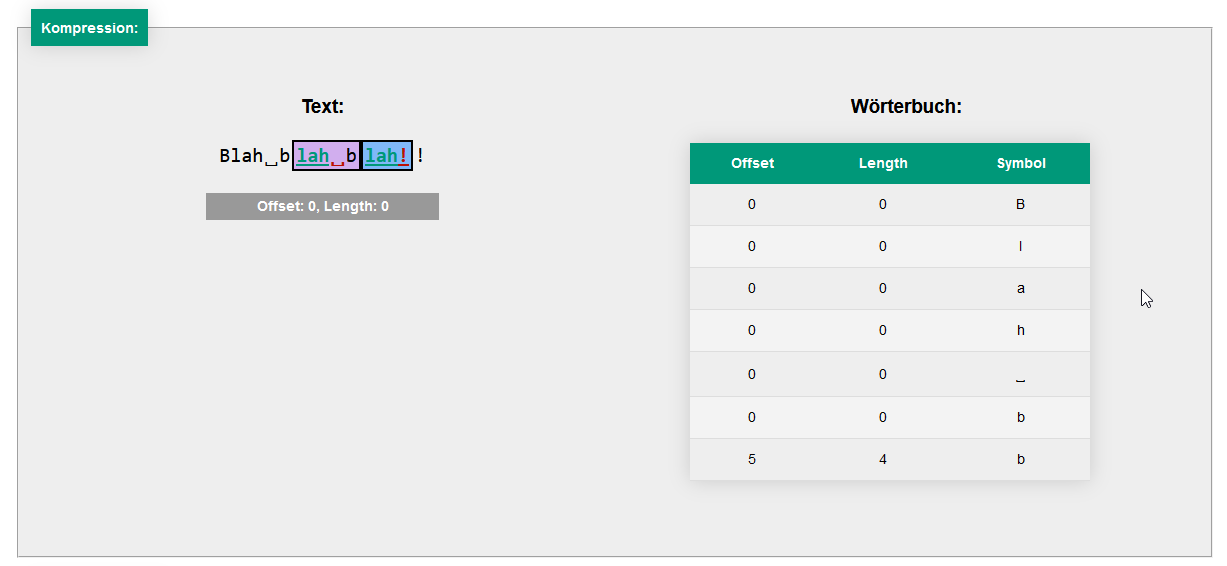
\includegraphics[scale=0.45]{pictures/Kompression.png}
    \caption{Kompressions-Bereich des Demonstrations-Kit mit Visualisierung.}
\end{figure}

\noindent
Der Dekompressions-Bereich veranschaulicht die Dekompression. Hier wird ebenfalls auf der linken Seite der Text angezeigt. Neu hinzugefügte Zeichen werden hier \underline{\textbf{Fett gedruckt und}} \underline{\textbf{unterstrichen}}. Zeichen die mittels Wörterbuch-Eintrag aus dem bereits decodierten Text geholt werden, sind \textcolor{htmlgreen}{\underline{\textbf{Grün}}} dargestellt. Auf der rechten Seite wird auch hier das Wörterbuch angezeigt. Dieses wird von der Kompression an die Dekompression übergeben. Der aktuell bearbeitete Eintrag wird \textcolor{gray}{\textbf{Grau}} hervorgehoben.

\begin{figure}[H]
    \centering
    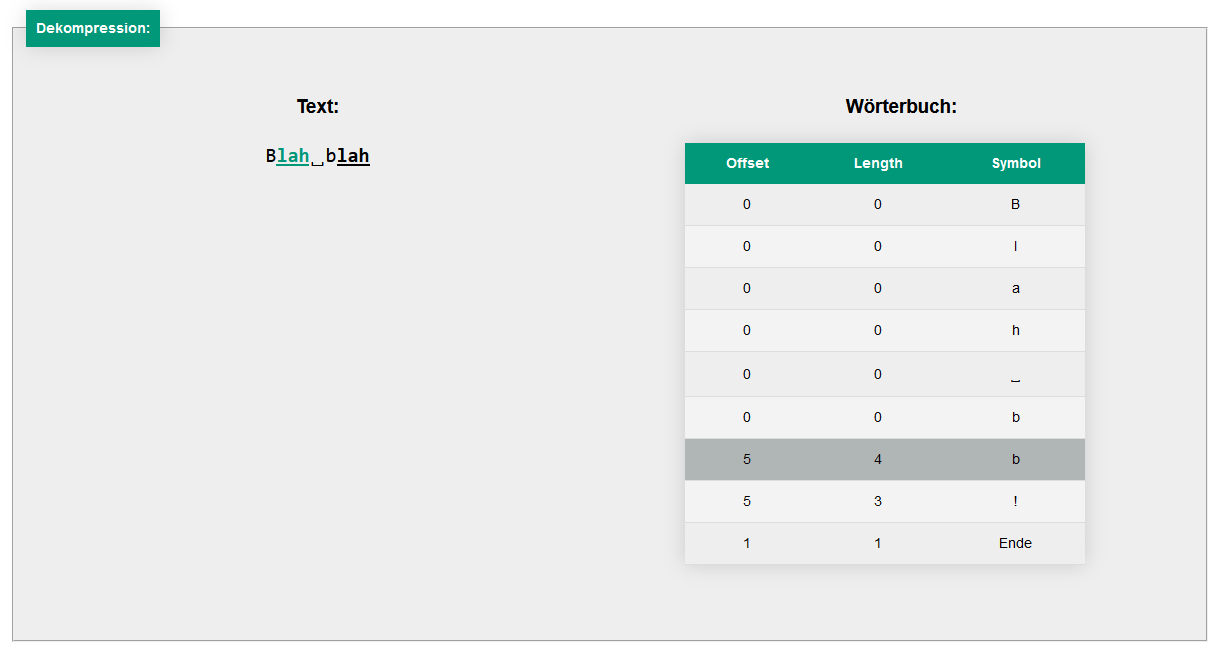
\includegraphics[scale=0.45]{pictures/Dekompression.png}
    \caption{Dekompressions-Bereich des Demonstrations-Kit mit Visualisierung.}
\end{figure}

\newpage
\section{Referenzen}
\bibliography{sources}
\bibliographystyle{alphadin}
\newpage

\section{Anhang}

\subsection{Kompressionsalgorithmus}
\label{sec:encode}
Der LZ77-Kompressionsalgorithmus implementiert in Javascript:
\begin{minted}{js}
function encode(string, searchBufferLength, lookaheadBufferLength) {
    let dictionary = new Dictionary();
    let i = 0;

    // loop through string:
    while (i < string.length) {
        let char = string.charAt(i);
        let offset = 0;
        let maxLength = 0;
        let j = i-1;

        // go backwards through searchbuffer:
        while (j >= 0 && i-j <= searchBufferLength) {
            if (string.charAt(i) == string.charAt(j)) {
                // match found
                let length = 1;
                // get length of match:
                while (length < lookaheadBufferLength && i+length < string.length) {
                    if (string.charAt(j+length) == string.charAt(i+length)) {
                        length++;
                    } else {
                        break;
                    }
                }
                // update if new best match:
                if (maxLength < length) {
                    maxLength = length;
                    offset = i-j;
                    if (i+length < string.length) {
                        char = string.charAt(i+length);
                    } else {
                        char = "Ende";
                    }
                }
            }
            j--; 
        }
        // add to dictionary:
        dictionary.addEntry(new Entry(offset, maxLength, char));

        // move sliding window:
        if (maxLength == 0) {
            i++;
        } else {
            i = i+maxLength+1;
        }
    }
    return dictionary;
}
\end{minted}

\subsection{Dekompressionsalogrithmus}
\label{sec:decode}
Der LZ77-Dekompressionsalgorithmus implementiert in Javascript:
\begin{minted}{js}
function decode(dictionary) {
    let decodedString = "";

    // loop through dictionary:
    for (let e = 0; e < dictionary.length; e++) {
        let offset = dictionary[e].getOffset();
        let length = dictionary[e].getLength();
        let char = dictionary[e].getNextSymbol();

        // put string together:
        if (length > 0) {
            for (let i = 0; i < length; i++) {
                decodedString += decodedString.charAt(decodedString.length - offset);
            }
        }
        if (char != "Ende") {
            decodedString += char;
        }
    }
    return decodedString;
}
\end{minted}

\end{document}
